% GENERATED FILE - do not hand-edit.
% Source of truth: data/calculus-reviewed/t-4.json in the zenith-website repo.
% Regenerate with: python3 scripts/build_calculus_tex.py
\documentclass[11pt]{article}
\usepackage[utf8]{inputenc}
\usepackage[T1]{fontenc}
\usepackage{amsmath,amssymb}
\usepackage{graphicx}
\usepackage[margin=1in]{geometry}
\graphicspath{{../..//}}
\setlength{\parindent}{0pt}
\setlength{\parskip}{0.6em}
\begin{document}
\section*{Chapter 4: Application of Differential Calculus --- Test T4}

\bigskip\noindent\textbf{T1.}\ The slope of the curve $y^3 - xy^2 = 16$ at the point where $y=2$ is
\begin{list}{}{\setlength{\leftmargin}{3em}\setlength{\labelwidth}{2.5em}\setlength{\itemsep}{0pt}\setlength{\topsep}{2pt}}
\item[(A)] $-\dfrac{1}{5}$
\item[(B)] $\dfrac{1}{5}$
\item[(C)] $-5$
\item[(D)] $5$
\end{list}

\bigskip\noindent\textbf{T2.}\ The slope of the curve $y^2 - xy - 5x = 1$ at the point $(0,-1)$ is
\begin{list}{}{\setlength{\leftmargin}{3em}\setlength{\labelwidth}{2.5em}\setlength{\itemsep}{0pt}\setlength{\topsep}{2pt}}
\item[(A)] $-1$
\item[(B)] $-2$
\item[(C)] $1$
\item[(D)] $2$
\end{list}

\bigskip\noindent\textbf{T3.}\ Find an equation of the tangent to $y=x\cos2x$ at $(\pi/4,0)$.
\begin{list}{}{\setlength{\leftmargin}{3em}\setlength{\labelwidth}{2.5em}\setlength{\itemsep}{0pt}\setlength{\topsep}{2pt}}
\item[(A)] $y=-\frac\pi2(x-\frac\pi4)$
\item[(B)] $y = \dfrac{\pi}{4}$
\item[(C)] $y = \dfrac{\pi}{4} - x$
\item[(D)] $y = x$
\end{list}

\bigskip\noindent\textbf{T4.}\ The tangent to the curve of $y = xe^{-2x}$ is horizontal when $x$ is equal to
\begin{list}{}{\setlength{\leftmargin}{3em}\setlength{\labelwidth}{2.5em}\setlength{\itemsep}{0pt}\setlength{\topsep}{2pt}}
\item[(A)] $0$
\item[(B)] $\dfrac{1}{2}$
\item[(C)] $-\dfrac{1}{2}$
\item[(D)] $\dfrac{1}{2e}$
\end{list}

\bigskip\noindent\textbf{T5.}\ The minimum value of the slope of the curve $y = x^5 + 2x^3 - 3x$ is
\begin{list}{}{\setlength{\leftmargin}{3em}\setlength{\labelwidth}{2.5em}\setlength{\itemsep}{0pt}\setlength{\topsep}{2pt}}
\item[(A)] $3$
\item[(B)] $9$
\item[(C)] $-3$
\item[(D)] $-9$
\end{list}

\bigskip\noindent\textbf{T6.}\ An equation of the tangent to the hyperbola $x^2-y^2=20$ at the point $(6,4)$ on the curve is
\begin{list}{}{\setlength{\leftmargin}{3em}\setlength{\labelwidth}{2.5em}\setlength{\itemsep}{0pt}\setlength{\topsep}{2pt}}
\item[(A)] $3x-2y+10=0$
\item[(B)] $y = \dfrac{3}{2}x$
\item[(C)] $y = \dfrac{3}{2}x - 5$
\item[(D)] $y = \dfrac{2}{3}x$
\end{list}

\bigskip\noindent\textbf{T7.}\ A tangent to the curve $y^2-xy+16=0$ is vertical when
\begin{list}{}{\setlength{\leftmargin}{3em}\setlength{\labelwidth}{2.5em}\setlength{\itemsep}{0pt}\setlength{\topsep}{2pt}}
\item[(A)] $y=0$
\item[(B)] $y = \pm 2$
\item[(C)] $y = \dfrac{1}{2}$
\item[(D)] $y = \pm 4$
\end{list}

\bigskip\noindent\textbf{T8.}\ The volume of a sphere is given by $V = \frac{4}{3}\pi r^3$. Use a tangent line to approximate the increase in volume, in cubic inches, when the radius of a sphere is increased from 4 to 4.1 inches.
\begin{list}{}{\setlength{\leftmargin}{3em}\setlength{\labelwidth}{2.5em}\setlength{\itemsep}{0pt}\setlength{\topsep}{2pt}}
\item[(A)] $0.04\pi$
\item[(B)] $0.16\pi$
\item[(C)] $1.6\pi$
\item[(D)] $6.4\pi$
\end{list}

\bigskip\noindent\textbf{T9.}\ When $x=4$, the equation $2x^2-y^3=24$ has the solution $y=2$. Using a tangent line to the graph of the curve, approximate $y$ when $x=4.03$.
\begin{list}{}{\setlength{\leftmargin}{3em}\setlength{\labelwidth}{2.5em}\setlength{\itemsep}{0pt}\setlength{\topsep}{2pt}}
\item[(A)] $1.6$
\item[(B)] $1.96$
\item[(C)] $2.04$
\item[(D)] $2.4$
\end{list}

\bigskip\noindent\textbf{T10.}\ If the side $e$ of a square is increased by 2\%, then the area is increased approximately
\begin{list}{}{\setlength{\leftmargin}{3em}\setlength{\labelwidth}{2.5em}\setlength{\itemsep}{0pt}\setlength{\topsep}{2pt}}
\item[(A)] $0.04e$
\item[(B)] $0.04e^2$
\item[(C)] $0.02e^2$
\item[(D)] $0.02e$
\end{list}

\bigskip\noindent\textbf{T11.}\ The edge of a cube has length 20 in., with a possible error of 2\%. The possible error, in cubic inches, in the volume of the cube is
\begin{list}{}{\setlength{\leftmargin}{3em}\setlength{\labelwidth}{2.5em}\setlength{\itemsep}{0pt}\setlength{\topsep}{2pt}}
\item[(A)] $4$
\item[(B)] $40$
\item[(C)] $240$
\item[(D)] $480$
\end{list}

\bigskip\noindent\textbf{T12.}\ The function $f(x) = x^4 - 8x^2$ has
\begin{list}{}{\setlength{\leftmargin}{3em}\setlength{\labelwidth}{2.5em}\setlength{\itemsep}{0pt}\setlength{\topsep}{2pt}}
\item[(A)] one local minimum and two local maxima
\item[(B)] one local minimum and no local maximum
\item[(C)] no local minimum and one local maximum
\item[(D)] two local minima and one local maximum
\end{list}

\bigskip\noindent\textbf{T13.}\ The number of inflection points on the graph of $f(x) = x^4 - 8x^2$ is
\begin{list}{}{\setlength{\leftmargin}{3em}\setlength{\labelwidth}{2.5em}\setlength{\itemsep}{0pt}\setlength{\topsep}{2pt}}
\item[(A)] $0$
\item[(B)] $1$
\item[(C)] $2$
\item[(D)] $3$
\end{list}

\bigskip\noindent\textbf{T14.}\ The maximum value of the function $y = -6\sqrt{3-x}$ is
\begin{list}{}{\setlength{\leftmargin}{3em}\setlength{\labelwidth}{2.5em}\setlength{\itemsep}{0pt}\setlength{\topsep}{2pt}}
\item[(A)] $0$
\item[(B)] $-6$
\item[(C)] $-3$
\item[(D)] $3$
\end{list}

\bigskip\noindent\textbf{T15.}\ The total number of local maximum and minimum points of the function whose derivative, for all $x$, is given by $f'(x) = x(x-4)^2(x+2)^4$ is
\begin{list}{}{\setlength{\leftmargin}{3em}\setlength{\labelwidth}{2.5em}\setlength{\itemsep}{0pt}\setlength{\topsep}{2pt}}
\item[(A)] $0$
\item[(B)] $1$
\item[(C)] $2$
\item[(D)] $3$
\end{list}

\bigskip\noindent\textbf{T16.}\ For which curve shown below are both $f'$ and $f''$ negative?
\begin{center}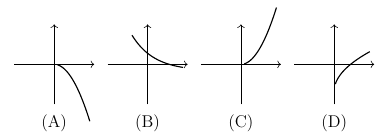
\includegraphics[width=0.6\linewidth]{data/calculus-figures/t4-curves.png}\end{center}
\begin{list}{}{\setlength{\leftmargin}{3em}\setlength{\labelwidth}{2.5em}\setlength{\itemsep}{0pt}\setlength{\topsep}{2pt}}
\item[(A)] Curve (A)
\item[(B)] Curve (B)
\item[(C)] Curve (C)
\item[(D)] Curve (D)
\end{list}

\bigskip\noindent\textbf{T17.}\ For which curve shown below is $f\prime\prime$ positive but $f\prime$ negative?
\begin{center}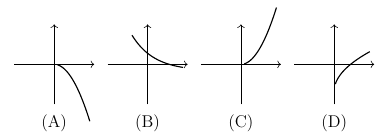
\includegraphics[width=0.6\linewidth]{data/calculus-figures/t4-curves.png}\end{center}
\begin{list}{}{\setlength{\leftmargin}{3em}\setlength{\labelwidth}{2.5em}\setlength{\itemsep}{0pt}\setlength{\topsep}{2pt}}
\item[(A)] Curve (A)
\item[(B)] Curve (B)
\item[(C)] Curve (C)
\item[(D)] Curve (D)
\end{list}

\bigskip\noindent\textbf{T18.}\ The position of a particle moving along a horizontal line is $s=t^3-9t^2+27t-5$. The object is moving to the right for
\begin{list}{}{\setlength{\leftmargin}{3em}\setlength{\labelwidth}{2.5em}\setlength{\itemsep}{0pt}\setlength{\topsep}{2pt}}
\item[(A)] $t < 3$
\item[(B)] all $t$ except $t=3$
\item[(C)] all $t$
\item[(D)] $t>3$
\end{list}

\bigskip\noindent\textbf{T19.}\ The position of a particle moving along a horizontal line is $s=t^3-9t^2+27t-5$. The minimum value of the speed is
\begin{list}{}{\setlength{\leftmargin}{3em}\setlength{\labelwidth}{2.5em}\setlength{\itemsep}{0pt}\setlength{\topsep}{2pt}}
\item[(A)] $0$
\item[(B)] $1$
\item[(C)] $2$
\item[(D)] $3$
\end{list}

\bigskip\noindent\textbf{T20.}\ The position of a particle moving along a horizontal line is $s=t^3-9t^2+27t-5$. The acceleration is positive
\begin{list}{}{\setlength{\leftmargin}{3em}\setlength{\labelwidth}{2.5em}\setlength{\itemsep}{0pt}\setlength{\topsep}{2pt}}
\item[(A)] when $t>3$
\item[(B)] for all $t$, $t \neq 3$
\item[(C)] when $t<3$
\item[(D)] for $1<t<3$
\end{list}

\bigskip\noindent\textbf{T21.}\ The position of a particle moving along a horizontal line is $s=t^3-9t^2+27t-5$. The speed of the particle is decreasing for
\begin{list}{}{\setlength{\leftmargin}{3em}\setlength{\labelwidth}{2.5em}\setlength{\itemsep}{0pt}\setlength{\topsep}{2pt}}
\item[(A)] $t<3$
\item[(B)] all $t$
\item[(C)] $t<1$ or $t>3$
\item[(D)] $t>3$
\end{list}

\bigskip\noindent\textbf{T22.}\ A particle moves along a horizontal line with position $s=t^4-10t^3+36t^2+3$ at time $t$. The particle is at rest when $t$ is equal to
\begin{list}{}{\setlength{\leftmargin}{3em}\setlength{\labelwidth}{2.5em}\setlength{\itemsep}{0pt}\setlength{\topsep}{2pt}}
\item[(A)] $2$ or $3$
\item[(B)] $0$
\item[(C)] $\dfrac{5}{2}$
\item[(D)] $0$, $2$, or $3$
\end{list}

\bigskip\noindent\textbf{T23.}\ A particle moves along a horizontal line with position $s=t^4-10t^3+36t^2+3$ at time $t$. The velocity, $v$, is increasing when
\begin{list}{}{\setlength{\leftmargin}{3em}\setlength{\labelwidth}{2.5em}\setlength{\itemsep}{0pt}\setlength{\topsep}{2pt}}
\item[(A)] $t>2$
\item[(B)] $2<t<3$
\item[(C)] $t<3$
\item[(D)] $t<2$ or $t>3$
\end{list}

\bigskip\noindent\textbf{T24.}\ A particle moves along a horizontal line with position $s=t^4-10t^3+36t^2+3$ at time $t$. The speed of the particle is increasing for
\begin{list}{}{\setlength{\leftmargin}{3em}\setlength{\labelwidth}{2.5em}\setlength{\itemsep}{0pt}\setlength{\topsep}{2pt}}
\item[(A)] $0<t<2$ or $t>3$
\item[(B)] $2<t<3$
\item[(C)] $t<3$
\item[(D)] $t<0$ or $t>3$
\end{list}

\bigskip\noindent\textbf{T25.}\ The displacement from the origin of a particle moving on a line is given by $s = 2t^4-8t^3$. The maximum displacement during the time interval $-2 \leq t \leq 4$ is
\begin{list}{}{\setlength{\leftmargin}{3em}\setlength{\labelwidth}{2.5em}\setlength{\itemsep}{0pt}\setlength{\topsep}{2pt}}
\item[(A)] $54$
\item[(B)] $6$
\item[(C)] $96$
\item[(D)] $32$
\end{list}

\bigskip\noindent\textbf{T26.}\ If a particle moves along a line according to the law $s = t^5+10t^4$, then the number of times it reverses direction is
\begin{list}{}{\setlength{\leftmargin}{3em}\setlength{\labelwidth}{2.5em}\setlength{\itemsep}{0pt}\setlength{\topsep}{2pt}}
\item[(A)] $0$
\item[(B)] $1$
\item[(C)] $2$
\item[(D)] $3$
\end{list}

\bigskip\noindent\textbf{T27.}\ The position vector of a moving point is $\mathbf R(t)=\langle4\cos(\pi t/4),3\sin(\pi t/4)\rangle$. A single equation in $x$ and $y$ for the path of the point is
\begin{list}{}{\setlength{\leftmargin}{3em}\setlength{\labelwidth}{2.5em}\setlength{\itemsep}{0pt}\setlength{\topsep}{2pt}}
\item[(A)] $x^2+y^2=25$
\item[(B)] $16x^2+9y^2=144$
\item[(C)] $3x^2+4y^2=25$
\item[(D)] $9x^2+16y^2=144$
\end{list}

\bigskip\noindent\textbf{T28.}\ The position vector of a moving point is $\mathbf R(t)=\langle4\cos(\pi t/4),3\sin(\pi t/4)\rangle$. When $t=4$, the speed of the particle is
\begin{list}{}{\setlength{\leftmargin}{3em}\setlength{\labelwidth}{2.5em}\setlength{\itemsep}{0pt}\setlength{\topsep}{2pt}}
\item[(A)] $\dfrac{3\pi}{4}$
\item[(B)] $3$
\item[(C)] $4$
\item[(D)] $\dfrac{\sqrt{7}}{4}\pi$
\end{list}

\bigskip\noindent\textbf{T29.}\ The position vector of a moving point is $\mathbf R(t)=\langle4\cos(\pi t/4),3\sin(\pi t/4)\rangle$. The magnitude of the acceleration when $t=4$ is
\begin{list}{}{\setlength{\leftmargin}{3em}\setlength{\labelwidth}{2.5em}\setlength{\itemsep}{0pt}\setlength{\topsep}{2pt}}
\item[(A)] $3$
\item[(B)] $\dfrac{\pi^2}{4}$
\item[(C)] $4$
\item[(D)] $\dfrac{3\pi^2}{16}$
\end{list}

\bigskip\noindent\textbf{T30.}\ The position vector of a moving point is $\mathbf R(t)=\langle4\cos(\pi t/4),3\sin(\pi t/4)\rangle$. At the point where $t=1$, the slope of the curve along which the particle moves is
\begin{list}{}{\setlength{\leftmargin}{3em}\setlength{\labelwidth}{2.5em}\setlength{\itemsep}{0pt}\setlength{\topsep}{2pt}}
\item[(A)] $-\dfrac{2\sqrt{2}}{3}$
\item[(B)] $-\dfrac{3}{4}$
\item[(C)] $\dfrac{3}{4}$
\item[(D)] $-\dfrac{4}{3}$
\end{list}

\bigskip\noindent\textbf{T31.}\ A balloon is being filled with helium at the rate of 8 ft$^3$/min. The rate, in square feet per minute, at which the surface area is increasing when the volume is $\dfrac{32\pi}{3}$ ft$^3$ is
\begin{list}{}{\setlength{\leftmargin}{3em}\setlength{\labelwidth}{2.5em}\setlength{\itemsep}{0pt}\setlength{\topsep}{2pt}}
\item[(A)] $8\pi$
\item[(B)] $2$
\item[(C)] $8$
\item[(D)] $1$
\end{list}

\bigskip\noindent\textbf{T32.}\ A circular conical reservoir, vertex down, has depth 30 ft and radius at the top 15 ft. Water is leaking out so that the surface is falling at the rate of $\dfrac{1}{3}$ ft/hr. The rate, in cubic feet per hour, at which the water is leaving the reservoir when the water is 6 ft deep is
\begin{list}{}{\setlength{\leftmargin}{3em}\setlength{\labelwidth}{2.5em}\setlength{\itemsep}{0pt}\setlength{\topsep}{2pt}}
\item[(A)] $3\pi$
\item[(B)] $6\pi$
\item[(C)] $\dfrac{1}{3\pi}$
\item[(D)] $\dfrac{1}{6\pi}$
\end{list}

\bigskip\noindent\textbf{T33.}\ A local minimum value of the function $y = \dfrac{e^x}{3x}$ is
\begin{list}{}{\setlength{\leftmargin}{3em}\setlength{\labelwidth}{2.5em}\setlength{\itemsep}{0pt}\setlength{\topsep}{2pt}}
\item[(A)] $\dfrac{1}{e}$
\item[(B)] $1$
\item[(C)] $-1$
\item[(D)] $\dfrac{e}{3}$
\end{list}

\bigskip\noindent\textbf{T34.}\ The area of the largest rectangle that can be drawn with one side along the $x$-axis and two vertices on the curve of $y = e^{-2x^2}$ is
\begin{list}{}{\setlength{\leftmargin}{3em}\setlength{\labelwidth}{2.5em}\setlength{\itemsep}{0pt}\setlength{\topsep}{2pt}}
\item[(A)] $\sqrt{\dfrac{2}{e}}$
\item[(B)] $\sqrt{\dfrac{1}{e}}$
\item[(C)] $\dfrac{2}{e}$
\item[(D)] $\dfrac{1}{\sqrt{2e}}$
\end{list}

\bigskip\noindent\textbf{T35.}\ A line with a negative slope is drawn through the point $(2,3)$ forming a right triangle with the positive $x$- and $y$-axes. The slope of the line forming the triangle of least area is
\begin{list}{}{\setlength{\leftmargin}{3em}\setlength{\labelwidth}{2.5em}\setlength{\itemsep}{0pt}\setlength{\topsep}{2pt}}
\item[(A)] $-1$
\item[(B)] $-\dfrac{3}{2}$
\item[(C)] $-2$
\item[(D)] $-3$
\end{list}

\bigskip\noindent\textbf{T36.}\ The point(s) on the curve $x^2-y^2=9$ closest to the point $(10,0)$ is (are)
\begin{list}{}{\setlength{\leftmargin}{3em}\setlength{\labelwidth}{2.5em}\setlength{\itemsep}{0pt}\setlength{\topsep}{2pt}}
\item[(A)] $(3,0)$
\item[(B)] $\left(\sqrt{13},\pm 2\right)$
\item[(C)] $(5,\pm 4)$
\item[(D)] $\left(\sqrt{109},\pm 10\right)$
\end{list}

\bigskip\noindent\textbf{T37.}\ The sum of the squares of two positive numbers is 300; their minimum product is
\begin{list}{}{\setlength{\leftmargin}{3em}\setlength{\labelwidth}{2.5em}\setlength{\itemsep}{0pt}\setlength{\topsep}{2pt}}
\item[(A)] $150$
\item[(B)] $30$
\item[(C)] $0$
\item[(D)] there is no minimum
\end{list}

\bigskip\noindent\textbf{T38.}\ The first-quadrant point on the curve $y^2x = 64$ that is closest to the point $(2,0)$ is
\begin{list}{}{\setlength{\leftmargin}{3em}\setlength{\labelwidth}{2.5em}\setlength{\itemsep}{0pt}\setlength{\topsep}{2pt}}
\item[(A)] $(4,4)$
\item[(B)] $\left(2,\sqrt{32}\right)$
\item[(C)] $\left(6,\sqrt{32/3}\right)$
\item[(D)] $(1,8)$
\end{list}

\bigskip\noindent\textbf{T39.}\ If $h$ is a small negative number, then the local linear approximation for $\sqrt[3]{64+h}$ is
\begin{list}{}{\setlength{\leftmargin}{3em}\setlength{\labelwidth}{2.5em}\setlength{\itemsep}{0pt}\setlength{\topsep}{2pt}}
\item[(A)] $4 + \dfrac{h}{48}$
\item[(B)] $4 - \dfrac{h}{48}$
\item[(C)] $\dfrac{h}{48}$
\item[(D)] $-\dfrac{h}{48}$
\end{list}

\bigskip\noindent\textbf{T40.}\ If $f(x) = xe^{-2x}$, then at $x=0$
\begin{list}{}{\setlength{\leftmargin}{3em}\setlength{\labelwidth}{2.5em}\setlength{\itemsep}{0pt}\setlength{\topsep}{2pt}}
\item[(A)] $f$ is increasing
\item[(B)] $f$ is decreasing
\item[(C)] $f$ has a relative maximum
\item[(D)] $f$ has a relative minimum
\end{list}

\bigskip\noindent\textbf{T41.}\ A function $f$ has a derivative for each $x$ such that $|x|<3$ and has a local minimum at $(3,-7)$. Which statement below must be true?
\begin{list}{}{\setlength{\leftmargin}{3em}\setlength{\labelwidth}{2.5em}\setlength{\itemsep}{0pt}\setlength{\topsep}{2pt}}
\item[(A)] $f'(3) = 0$
\item[(B)] $f'$ exists at $x=3$
\item[(C)] $f'(x)<0$ if $x<3$, $f'(x)>0$ if $x>3$
\item[(D)] none of the preceding is necessarily true
\end{list}

\bigskip\noindent\textbf{T42.}\ The height of a rectangular box is 10 in. Its length increases at the rate of 3 in./sec; its width decreases at the rate of 5 in./sec. When the length is 6 in. and the width is 9 in., the rate, in cubic inches per second, at which the volume of the box is changing is
\begin{list}{}{\setlength{\leftmargin}{3em}\setlength{\labelwidth}{2.5em}\setlength{\itemsep}{0pt}\setlength{\topsep}{2pt}}
\item[(A)] $30$
\item[(B)] $-30$
\item[(C)] $300$
\item[(D)] $-300$
\end{list}

\bigskip\noindent\textbf{T43.}\ The tangent to the curve $x^3+x^2y+5y=17$ at the point $(2,1)$ has slope
\begin{list}{}{\setlength{\leftmargin}{3em}\setlength{\labelwidth}{2.5em}\setlength{\itemsep}{0pt}\setlength{\topsep}{2pt}}
\item[(A)] $-2$
\item[(B)] $-\dfrac{16}{9}$
\item[(C)] $-\dfrac{9}{16}$
\item[(D)] $\dfrac{16}{9}$
\end{list}

\bigskip\noindent\textbf{T44.}\ If $f(x) = ax^6+bx^2$ and $ab>0$, then
\begin{list}{}{\setlength{\leftmargin}{3em}\setlength{\labelwidth}{2.5em}\setlength{\itemsep}{0pt}\setlength{\topsep}{2pt}}
\item[(A)] the curve has no horizontal tangents
\item[(B)] the curve is concave up for all $x$
\item[(C)] the curve has no inflection point
\item[(D)] none of the preceding is necessarily true
\end{list}

\bigskip\noindent\textbf{T45.}\ A function $f$ is continuous and differentiable on the interval $[0,4]$, where $f'$ is positive but $f''$ is negative. Which table could represent points on $f$?
\begin{list}{}{\setlength{\leftmargin}{3em}\setlength{\labelwidth}{2.5em}\setlength{\itemsep}{0pt}\setlength{\topsep}{2pt}}
\item[(A)] $\begin{array}{c|rrrrr}x&0&1&2&3&4\\y&5&7&9&11&13\end{array}$
\item[(B)] $\begin{array}{c|rrrrr}x&0&1&2&3&4\\y&5&7&10&14&19\end{array}$
\item[(C)] $\begin{array}{c|rrrrr}x&0&1&2&3&4\\y&5&13&19&23&25\end{array}$
\item[(D)] $\begin{array}{c|rrrrr}x&0&1&2&3&4\\y&5&9&16&19&21\end{array}$
\end{list}

\bigskip\noindent\textbf{T46.}\ An equation of the tangent to the curve with parametric equations $x = 3t+1$, $y = 4-t^3$ at the point where $t=1$ is
\begin{list}{}{\setlength{\leftmargin}{3em}\setlength{\labelwidth}{2.5em}\setlength{\itemsep}{0pt}\setlength{\topsep}{2pt}}
\item[(A)] $x+y=7$
\item[(B)] $3x+2y=18$
\item[(C)] $2x+3y=17$
\item[(D)] $x-2y=-2$
\end{list}

\bigskip\noindent\textbf{T47.}\ Given the function $f(x) = \sqrt[3]{x}$, it is known that $f(125) = 5$. Using the tangent line to the graph of $f(x)$, approximately how much less than 5 is $\sqrt[3]{124}$?
\begin{list}{}{\setlength{\leftmargin}{3em}\setlength{\labelwidth}{2.5em}\setlength{\itemsep}{0pt}\setlength{\topsep}{2pt}}
\item[(A)] $\dfrac{1}{75}$
\item[(B)] $\dfrac{1}{25}$
\item[(C)] $\dfrac{1}{5}$
\item[(D)] $\dfrac{3}{5}$
\end{list}

\bigskip\noindent\textbf{T48.}\ The best linear approximation for $f(x) = \cot x$ near $x = \dfrac{\pi}{4}$ is $y=$
\begin{list}{}{\setlength{\leftmargin}{3em}\setlength{\labelwidth}{2.5em}\setlength{\itemsep}{0pt}\setlength{\topsep}{2pt}}
\item[(A)] $1 + \dfrac{1}{2}\left(x-\dfrac{\pi}{4}\right)$
\item[(B)] $1 + \left(x-\dfrac{\pi}{4}\right)$
\item[(C)] $1 - 2\left(x-\dfrac{\pi}{4}\right)$
\item[(D)] $1 + 2\left(x-\dfrac{\pi}{4}\right)$
\end{list}

\bigskip\noindent\textbf{T49.}\ Given $f(x) = e^{kx}$, approximate $f(h)$, where $h$ is near zero, using a tangent-line approximation. $f(h) \approx$
\begin{list}{}{\setlength{\leftmargin}{3em}\setlength{\labelwidth}{2.5em}\setlength{\itemsep}{0pt}\setlength{\topsep}{2pt}}
\item[(A)] $k$
\item[(B)] $kh$
\item[(C)] $1+k$
\item[(D)] $1+kh$
\end{list}

\bigskip\noindent\textbf{T50.}\ If $f(x) = cx^2+dx+e$ for the function shown in the graph, then
\begin{center}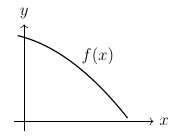
\includegraphics[width=0.6\linewidth]{data/calculus-figures/t4-quadratic.png}\end{center}
\begin{list}{}{\setlength{\leftmargin}{3em}\setlength{\labelwidth}{2.5em}\setlength{\itemsep}{0pt}\setlength{\topsep}{2pt}}
\item[(A)] $c$, $d$, and $e$ are all positive
\item[(B)] $c>0$, $d<0$, $e>0$
\item[(C)] $c<0$, $d>0$, $e>0$
\item[(D)] $c<0$, $d<0$, $e>0$
\end{list}

\bigskip\noindent\textbf{T51.}\ Given $f(x) = \log_{10}x$ and $\log_{10}(104) \approx 2.0170$, which is closest to $f'(100)$?
\begin{list}{}{\setlength{\leftmargin}{3em}\setlength{\labelwidth}{2.5em}\setlength{\itemsep}{0pt}\setlength{\topsep}{2pt}}
\item[(A)] $0.0043$
\item[(B)] $0.0085$
\item[(C)] $0.01$
\item[(D)] $1.0043$
\end{list}

\bigskip\noindent\textbf{TB1.}\ The point on the curve $y = \sqrt{3x-2}$ at which the tangent is parallel to the line $3x-8y=10$ is
\begin{list}{}{\setlength{\leftmargin}{3em}\setlength{\labelwidth}{2.5em}\setlength{\itemsep}{0pt}\setlength{\topsep}{2pt}}
\item[(A)] $(6,4)$
\item[(B)] $(2,2)$
\item[(C)] $(3,\sqrt{7})$
\item[(D)] $(1,1)$
\end{list}

\bigskip\noindent\textbf{TB2.}\ An equation of the tangent to the curve $x^2 = 6y$ at the point on the curve where $x=-3$ is
\begin{list}{}{\setlength{\leftmargin}{3em}\setlength{\labelwidth}{2.5em}\setlength{\itemsep}{0pt}\setlength{\topsep}{2pt}}
\item[(A)] $2x+2y+3=0$
\item[(B)] $2x-2y+3=0$
\item[(C)] $x+y-3=0$
\item[(D)] $x-y+3=0$
\end{list}

\bigskip\noindent\textbf{TB3.}\ The table shows the velocity at time $t$ of an object moving along a line. Estimate the acceleration (in ft/sec$^2$) at $t=6$ sec. $\begin{array}{c|rrrr}t\ (\mathrm{sec})&0&4&8&10\\v\ (\mathrm{ft/sec})&24&20&12&0\end{array}$
\begin{list}{}{\setlength{\leftmargin}{3em}\setlength{\labelwidth}{2.5em}\setlength{\itemsep}{0pt}\setlength{\topsep}{2pt}}
\item[(A)] $-8$
\item[(B)] $-2$
\item[(C)] $2$
\item[(D)] $8$
\end{list}

\bigskip\noindent\textbf{TB4.}\ The figure shows $f\prime$ on $[0,8]$. From the graph it follows that
\begin{center}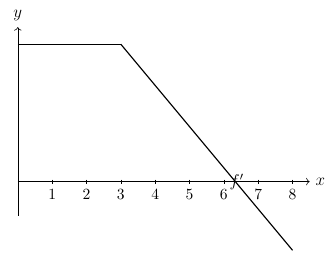
\includegraphics[width=0.6\linewidth]{data/calculus-figures/t4-fprime-linear.png}\end{center}
\begin{list}{}{\setlength{\leftmargin}{3em}\setlength{\labelwidth}{2.5em}\setlength{\itemsep}{0pt}\setlength{\topsep}{2pt}}
\item[(A)] $f$ is discontinuous at $x=3$
\item[(B)] $f$ is decreasing for $3<x<8$
\item[(C)] $f(5) < f(0)$
\item[(D)] $f(1) < f(2)$
\end{list}

\bigskip\noindent\textbf{TB5.}\ The figure shows $f\prime$ on $[0,8]$. Which statement best describes $f$ at $x=5$?
\begin{center}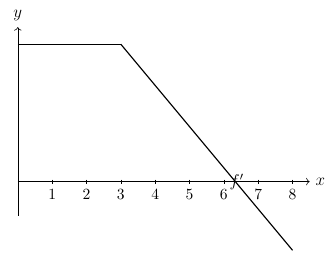
\includegraphics[width=0.6\linewidth]{data/calculus-figures/t4-fprime-linear.png}\end{center}
\begin{list}{}{\setlength{\leftmargin}{3em}\setlength{\labelwidth}{2.5em}\setlength{\itemsep}{0pt}\setlength{\topsep}{2pt}}
\item[(A)] $f$ has a root.
\item[(B)] $f$ has a maximum.
\item[(C)] $f$ has a minimum.
\item[(D)] $f$ is increasing and concave down near $x=5$.
\end{list}

\bigskip\noindent\textbf{TB6.}\ The figure shows $f\prime$ on $[0,8]$. For which interval is the graph of $f$ concave downward?
\begin{center}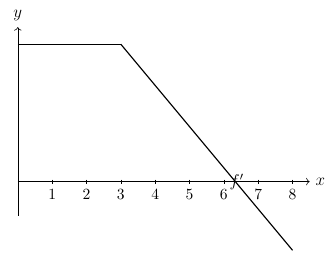
\includegraphics[width=0.6\linewidth]{data/calculus-figures/t4-fprime-linear.png}\end{center}
\begin{list}{}{\setlength{\leftmargin}{3em}\setlength{\labelwidth}{2.5em}\setlength{\itemsep}{0pt}\setlength{\topsep}{2pt}}
\item[(A)] $(0,3)$
\item[(B)] $(3,5)$
\item[(C)] $(5,8)$
\item[(D)] $(3,8)$
\end{list}

\bigskip\noindent\textbf{TB7.}\ The figure shows velocity in ft/sec on $0\le t\le6$. The object attains its maximum speed when $t=$
\begin{center}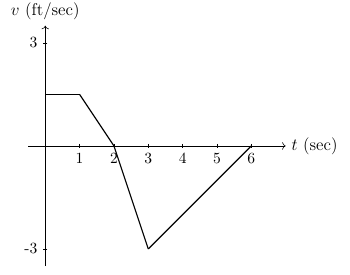
\includegraphics[width=0.6\linewidth]{data/calculus-figures/t4-velocity.png}\end{center}
\begin{list}{}{\setlength{\leftmargin}{3em}\setlength{\labelwidth}{2.5em}\setlength{\itemsep}{0pt}\setlength{\topsep}{2pt}}
\item[(A)] $0$
\item[(B)] $1$
\item[(C)] $2$
\item[(D)] $3$
\end{list}

\bigskip\noindent\textbf{TB8.}\ The figure shows velocity in ft/sec on $0\le t\le6$. The speed of the object is increasing during the time interval
\begin{center}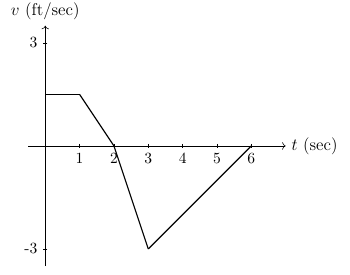
\includegraphics[width=0.6\linewidth]{data/calculus-figures/t4-velocity.png}\end{center}
\begin{list}{}{\setlength{\leftmargin}{3em}\setlength{\labelwidth}{2.5em}\setlength{\itemsep}{0pt}\setlength{\topsep}{2pt}}
\item[(A)] $(1,2)$
\item[(B)] $(0,2)$
\item[(C)] $(2,3)$
\item[(D)] $(3,6)$
\end{list}

\bigskip\noindent\textbf{TB9.}\ The figure shows velocity in ft/sec on $0\le t\le6$. The acceleration of the object is positive during the time interval
\begin{center}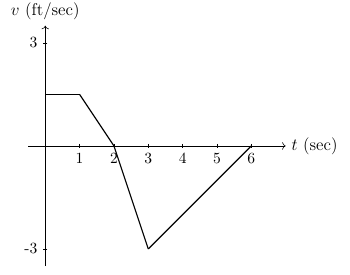
\includegraphics[width=0.6\linewidth]{data/calculus-figures/t4-velocity.png}\end{center}
\begin{list}{}{\setlength{\leftmargin}{3em}\setlength{\labelwidth}{2.5em}\setlength{\itemsep}{0pt}\setlength{\topsep}{2pt}}
\item[(A)] $(1,2)$
\item[(B)] $(0,2)$
\item[(C)] $(2,3)$
\item[(D)] $(3,6)$
\end{list}

\bigskip\noindent\textbf{TB10.}\ The figure shows velocity in ft/sec on $0\le t\le6$. How many times on $0<t<6$ is the object's acceleration undefined?
\begin{center}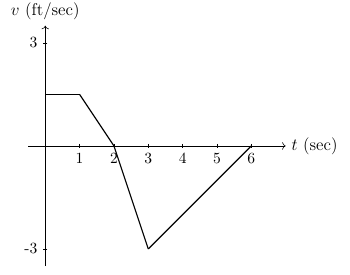
\includegraphics[width=0.6\linewidth]{data/calculus-figures/t4-velocity.png}\end{center}
\begin{list}{}{\setlength{\leftmargin}{3em}\setlength{\labelwidth}{2.5em}\setlength{\itemsep}{0pt}\setlength{\topsep}{2pt}}
\item[(A)] none
\item[(B)] $1$
\item[(C)] $2$
\item[(D)] $3$
\end{list}

\bigskip\noindent\textbf{TB11.}\ The figure shows velocity in ft/sec on $0\le t\le6$. During $2<t<3$, the object's acceleration (in ft/sec$^2$) is
\begin{center}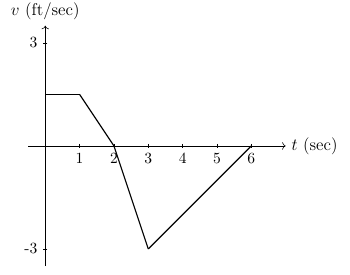
\includegraphics[width=0.6\linewidth]{data/calculus-figures/t4-velocity.png}\end{center}
\begin{list}{}{\setlength{\leftmargin}{3em}\setlength{\labelwidth}{2.5em}\setlength{\itemsep}{0pt}\setlength{\topsep}{2pt}}
\item[(A)] $-12$
\item[(B)] $-3$
\item[(C)] $6$
\item[(D)] $12$
\end{list}

\bigskip\noindent\textbf{TB12.}\ The figure shows velocity in ft/sec on $0\le t\le6$. The object is farthest to the right when $t=$
\begin{center}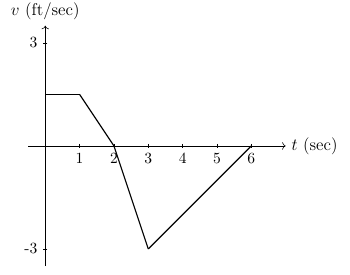
\includegraphics[width=0.6\linewidth]{data/calculus-figures/t4-velocity.png}\end{center}
\begin{list}{}{\setlength{\leftmargin}{3em}\setlength{\labelwidth}{2.5em}\setlength{\itemsep}{0pt}\setlength{\topsep}{2pt}}
\item[(A)] $0$
\item[(B)] $1$
\item[(C)] $2$
\item[(D)] $6$
\end{list}

\bigskip\noindent\textbf{TB13.}\ The figure shows velocity in ft/sec on $0\le t\le6$. The object's average acceleration (in ft/sec$^2$) for the interval $0 \leq t \leq 3$ is
\begin{center}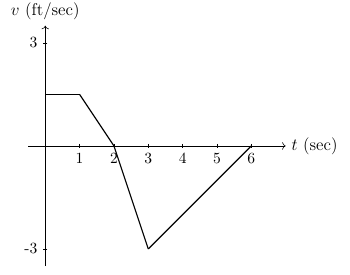
\includegraphics[width=0.6\linewidth]{data/calculus-figures/t4-velocity.png}\end{center}
\begin{list}{}{\setlength{\leftmargin}{3em}\setlength{\labelwidth}{2.5em}\setlength{\itemsep}{0pt}\setlength{\topsep}{2pt}}
\item[(A)] $-18$
\item[(B)] $-6$
\item[(C)] $-4$
\item[(D)] $-1.5$
\end{list}

\bigskip\noindent\textbf{TB14.}\ The line $y=12x+k$ is tangent to the curve $y=x^3$ when $k$ is equal to
\begin{list}{}{\setlength{\leftmargin}{3em}\setlength{\labelwidth}{2.5em}\setlength{\itemsep}{0pt}\setlength{\topsep}{2pt}}
\item[(A)] $1$ or $-1$
\item[(B)] $2$ or $-2$
\item[(C)] $8$ or $-8$
\item[(D)] $16$ or $-16$
\end{list}

\bigskip\noindent\textbf{TB15.}\ The two tangents that can be drawn from the point $(4,7)$ to the parabola $y=x^2$ have slopes
\begin{list}{}{\setlength{\leftmargin}{3em}\setlength{\labelwidth}{2.5em}\setlength{\itemsep}{0pt}\setlength{\topsep}{2pt}}
\item[(A)] $1$ and $7$
\item[(B)] $2$ and $14$
\item[(C)] $4$ and $28$
\item[(D)] $2$ and $7$
\end{list}

\bigskip\noindent\textbf{TB16.}\ The table shows the velocity at various times of an object moving along a line. An estimate of its acceleration (in ft/sec$^2$) at $t=1$ is $\begin{array}{c|rrrr}t\ (\mathrm{sec})&1.0&1.5&2.1&2.5\\v\ (\mathrm{ft/sec})&10.0&10.8&11.28&11.5\end{array}$
\begin{list}{}{\setlength{\leftmargin}{3em}\setlength{\labelwidth}{2.5em}\setlength{\itemsep}{0pt}\setlength{\topsep}{2pt}}
\item[(A)] $0.8$
\item[(B)] $1.0$
\item[(C)] $1.2$
\item[(D)] $1.6$
\end{list}

\bigskip\noindent\textbf{TB17.}\ For $0<x<5$, $f\prime(x)=x\sin x-2\cos x$. $f$ has a local maximum when $x$ is approximately
\begin{list}{}{\setlength{\leftmargin}{3em}\setlength{\labelwidth}{2.5em}\setlength{\itemsep}{0pt}\setlength{\topsep}{2pt}}
\item[(A)] $1.077$
\item[(B)] $2.456$
\item[(C)] $3.644$
\item[(D)] $4.100$
\end{list}

\bigskip\noindent\textbf{TB18.}\ For $0<x<5$, $f\prime(x)=x\sin x-2\cos x$. The graph of $f$ has a point of inflection when $x$ is approximately
\begin{list}{}{\setlength{\leftmargin}{3em}\setlength{\labelwidth}{2.5em}\setlength{\itemsep}{0pt}\setlength{\topsep}{2pt}}
\item[(A)] $1.077$
\item[(B)] $2.456$
\item[(C)] $3.644$
\item[(D)] $4.100$
\end{list}

\bigskip\noindent\textbf{TB19.}\ A particle has position $x=3t$, $y=6t-t^2$. The particle moves along
\begin{list}{}{\setlength{\leftmargin}{3em}\setlength{\labelwidth}{2.5em}\setlength{\itemsep}{0pt}\setlength{\topsep}{2pt}}
\item[(A)] an ellipse
\item[(B)] a hyperbola
\item[(C)] a line
\item[(D)] a parabola
\end{list}

\bigskip\noindent\textbf{TB20.}\ A particle has position $x=3t$, $y=6t-t^2$. The speed of the particle at any time $t$ is
\begin{list}{}{\setlength{\leftmargin}{3em}\setlength{\labelwidth}{2.5em}\setlength{\itemsep}{0pt}\setlength{\topsep}{2pt}}
\item[(A)] $\sqrt{10-2t}$
\item[(B)] $\sqrt{4t^2-24t+45}$
\item[(C)] $2\sqrt{t^2-3t+10}$
\item[(D)] $2(|5-t|)$
\end{list}

\bigskip\noindent\textbf{TB21.}\ A particle has position $x=3t$, $y=6t-t^2$. The minimum speed of the particle is
\begin{list}{}{\setlength{\leftmargin}{3em}\setlength{\labelwidth}{2.5em}\setlength{\itemsep}{0pt}\setlength{\topsep}{2pt}}
\item[(A)] $0$
\item[(B)] $1$
\item[(C)] $3$
\item[(D)] $4$
\end{list}

\bigskip\noindent\textbf{TB22.}\ A particle has position $x=3t$, $y=6t-t^2$. The acceleration of the particle
\begin{list}{}{\setlength{\leftmargin}{3em}\setlength{\labelwidth}{2.5em}\setlength{\itemsep}{0pt}\setlength{\topsep}{2pt}}
\item[(A)] depends on $t$
\item[(B)] is always directed upward
\item[(C)] is constant both in magnitude and in direction
\item[(D)] never exceeds 1 in magnitude
\end{list}

\bigskip\noindent\textbf{TB23.}\ If a particle moves along a curve with constant speed, then
\begin{list}{}{\setlength{\leftmargin}{3em}\setlength{\labelwidth}{2.5em}\setlength{\itemsep}{0pt}\setlength{\topsep}{2pt}}
\item[(A)] the magnitude of its acceleration must equal zero
\item[(B)] the direction of acceleration must be constant
\item[(C)] the curve along which the particle moves must be a straight line
\item[(D)] its velocity and acceleration vectors must be perpendicular
\end{list}

\bigskip\noindent\textbf{TB24.}\ A particle is moving on the curve of $y = 3x - \ln x$ so that $\dfrac{dx}{dt} = -3$ at all times $t$. At the point $(1,3)$, $\dfrac{dy}{dt}$ is
\begin{list}{}{\setlength{\leftmargin}{3em}\setlength{\labelwidth}{2.5em}\setlength{\itemsep}{0pt}\setlength{\topsep}{2pt}}
\item[(A)] $-6$
\item[(B)] $-3$
\item[(C)] $3$
\item[(D)] $6$
\end{list}

\bigskip\noindent\textbf{TB25.}\ A particle moves on $r=8\cos2\theta$, with $d\theta/dt=1/4$ radian/sec when $\theta=\pi/6$. At $\theta = \dfrac{\pi}{6}$, find the rate of change (in units per second) of the particle's distance from the origin.
\begin{list}{}{\setlength{\leftmargin}{3em}\setlength{\labelwidth}{2.5em}\setlength{\itemsep}{0pt}\setlength{\topsep}{2pt}}
\item[(A)] $-8\sqrt{3}$
\item[(B)] $-2\sqrt{3}$
\item[(C)] $2\sqrt{3}$
\item[(D)] $8\sqrt{3}$
\end{list}

\bigskip\noindent\textbf{TB26.}\ A particle moves on $r=8\cos2\theta$, with $d\theta/dt=1/4$ radian/sec when $\theta=\pi/6$. At $\theta = \dfrac{\pi}{6}$, what is the horizontal component of the particle's velocity?
\begin{list}{}{\setlength{\leftmargin}{3em}\setlength{\labelwidth}{2.5em}\setlength{\itemsep}{0pt}\setlength{\topsep}{2pt}}
\item[(A)] $-\dfrac{21}{2}$
\item[(B)] $-\dfrac{7}{2}$
\item[(C)] $-2$
\item[(D)] $\dfrac{1}{2}$
\end{list}

\bigskip\noindent\textbf{TB27.}\ The figure shows $f\prime$ on $[0,5]$. $f$ has a local minimum at $x=$
\begin{center}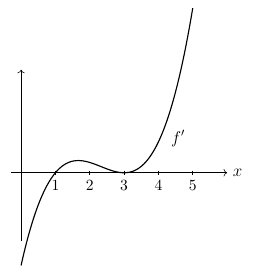
\includegraphics[width=0.6\linewidth]{data/calculus-figures/t4-fprime-cubic.png}\end{center}
\begin{list}{}{\setlength{\leftmargin}{3em}\setlength{\labelwidth}{2.5em}\setlength{\itemsep}{0pt}\setlength{\topsep}{2pt}}
\item[(A)] $0$
\item[(B)] $1$
\item[(C)] $2$
\item[(D)] $3$
\end{list}

\bigskip\noindent\textbf{TB28.}\ The figure shows $f\prime$ on $[0,5]$. The graph of $f$ has a point of inflection at $x=$
\begin{center}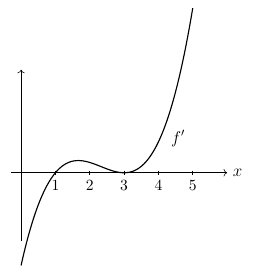
\includegraphics[width=0.6\linewidth]{data/calculus-figures/t4-fprime-cubic.png}\end{center}
\begin{list}{}{\setlength{\leftmargin}{3em}\setlength{\labelwidth}{2.5em}\setlength{\itemsep}{0pt}\setlength{\topsep}{2pt}}
\item[(A)] $1$ only
\item[(B)] $\dfrac{5}{3}$ only
\item[(C)] $3$ only
\item[(D)] $\dfrac{5}{3}$ and $3$ only
\end{list}

\bigskip\noindent\textbf{TB29.}\ It follows from the graph of $f'$, shown above, that
\begin{center}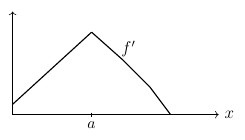
\includegraphics[width=0.6\linewidth]{data/calculus-figures/t4-fprime-corner.png}\end{center}
\begin{list}{}{\setlength{\leftmargin}{3em}\setlength{\labelwidth}{2.5em}\setlength{\itemsep}{0pt}\setlength{\topsep}{2pt}}
\item[(A)] $f$ is not continuous at $x=a$
\item[(B)] $f$ is continuous but not differentiable at $x=a$
\item[(C)] $f$ has a relative maximum at $x=a$
\item[(D)] The graph of $f$ has a point of inflection at $x=a$
\end{list}

\bigskip\noindent\textbf{TB30.}\ A vertical circular cylinder has radius $r$ ft and height $h$ ft. If the height and radius both increase at the constant rate of 3 ft/sec, then the rate, in square feet per second, at which the lateral surface area increases is
\begin{list}{}{\setlength{\leftmargin}{3em}\setlength{\labelwidth}{2.5em}\setlength{\itemsep}{0pt}\setlength{\topsep}{2pt}}
\item[(A)] $6\pi r$
\item[(B)] $3\pi(r+h)$
\item[(C)] $6\pi(r+h)$
\item[(D)] $6\pi h$
\end{list}

\bigskip\noindent\textbf{TB31.}\ A tangent drawn to the parabola $y=9-x^2$ at the point $(2,5)$ forms a right triangle with the coordinate axes. The area of the triangle is
\begin{list}{}{\setlength{\leftmargin}{3em}\setlength{\labelwidth}{2.5em}\setlength{\itemsep}{0pt}\setlength{\topsep}{2pt}}
\item[(A)] $\dfrac{169}{16}$
\item[(B)] $\dfrac{169}{8}$
\item[(C)] $\dfrac{13}{4}$
\item[(D)] $\dfrac{13}{2}$
\end{list}

\bigskip\noindent\textbf{TB32.}\ Two cars are traveling along perpendicular roads, car $A$ at 30 mph and car $B$ at 90 mph. At noon, when car $A$ reaches the intersection, car $B$ is 130 miles away, and moving toward the intersection. At 1 P.M. the rate, in miles per hour, at which the distance between the cars is changing is
\begin{list}{}{\setlength{\leftmargin}{3em}\setlength{\labelwidth}{2.5em}\setlength{\itemsep}{0pt}\setlength{\topsep}{2pt}}
\item[(A)] $-90$
\item[(B)] $-54$
\item[(C)] $54$
\item[(D)] $90$
\end{list}

\bigskip\noindent\textbf{TB33.}\ Two cars are traveling along perpendicular roads, car $A$ at 30 mph and car $B$ at 90 mph. At noon, when car $A$ reaches the intersection, car $B$ is 130 miles away and moving toward the intersection. If $t$ represents the time, in hours, traveled after noon, then the cars are closest together when $t$ is
\begin{list}{}{\setlength{\leftmargin}{3em}\setlength{\labelwidth}{2.5em}\setlength{\itemsep}{0pt}\setlength{\topsep}{2pt}}
\item[(A)] $1.038$
\item[(B)] $1.077$
\item[(C)] $1.3$
\item[(D)] $1.8$
\end{list}

\bigskip\noindent\textbf{TB34.}\ The figure shows velocity in ft/sec on $0\le t\le12$. For what $t$ does this object attain its maximum acceleration?
\begin{center}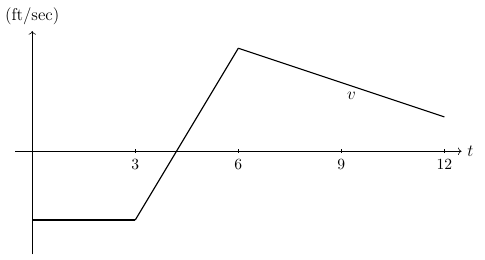
\includegraphics[width=0.6\linewidth]{data/calculus-figures/t4-velocity-long.png}\end{center}
\begin{list}{}{\setlength{\leftmargin}{3em}\setlength{\labelwidth}{2.5em}\setlength{\itemsep}{0pt}\setlength{\topsep}{2pt}}
\item[(A)] $0<t<3$
\item[(B)] $3<t<6$
\item[(C)] $t=4.5$
\item[(D)] $t=6$
\end{list}

\bigskip\noindent\textbf{TB35.}\ The figure shows velocity in ft/sec on $0\le t\le12$. The object reverses direction at $t=$
\begin{center}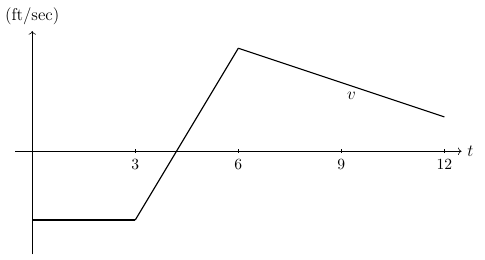
\includegraphics[width=0.6\linewidth]{data/calculus-figures/t4-velocity-long.png}\end{center}
\begin{list}{}{\setlength{\leftmargin}{3em}\setlength{\labelwidth}{2.5em}\setlength{\itemsep}{0pt}\setlength{\topsep}{2pt}}
\item[(A)] $3$ only
\item[(B)] $4.2$ only
\item[(C)] $6$ only
\item[(D)] $4.5$ and $6$ only
\end{list}

\bigskip\noindent\textbf{TB36.}\ Given that $f'$ is continuous and differentiable on $(0,4)$, with $f'(1)=0$ (where $f'$ changes from positive to negative) and $f'(3)=0$ (where $f'$ changes from negative to positive), which must be true of the graph of $f$?
\begin{list}{}{\setlength{\leftmargin}{3em}\setlength{\labelwidth}{2.5em}\setlength{\itemsep}{0pt}\setlength{\topsep}{2pt}}
\item[(A)] $f$ has a sharp corner at $x=1$
\item[(B)] $f$ has a local maximum at $x=1$ and a local minimum at $x=3$
\item[(C)] $f$ has a local minimum at $x=1$ and a local maximum at $x=3$
\item[(D)] $f$ is not differentiable at $x=1$ or $x=3$
\end{list}

\bigskip\noindent\textbf{TB37.}\ Given $f(3)=15$ and $f\prime(3)=6$, find the local linearization of $f$ at $x=3$.
\begin{list}{}{\setlength{\leftmargin}{3em}\setlength{\labelwidth}{2.5em}\setlength{\itemsep}{0pt}\setlength{\topsep}{2pt}}
\item[(A)] $\dfrac{x}{3}+14$
\item[(B)] $\dfrac{x}{3}+13$
\item[(C)] $6x-3$
\item[(D)] $6x+9$
\end{list}

\bigskip\noindent\textbf{TB38.}\ Use the labeled curve in the figure. At which labeled point do both $\dfrac{dy}{dx}$ and $\dfrac{d^2y}{dx^2}$ equal zero?
\begin{center}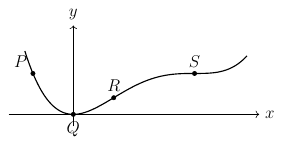
\includegraphics[width=0.6\linewidth]{data/calculus-figures/t4-labeled-curve.png}\end{center}
\begin{list}{}{\setlength{\leftmargin}{3em}\setlength{\labelwidth}{2.5em}\setlength{\itemsep}{0pt}\setlength{\topsep}{2pt}}
\item[(A)] $P$
\item[(B)] $Q$
\item[(C)] $R$
\item[(D)] $S$
\end{list}

\bigskip\noindent\textbf{TB39.}\ Use the labeled curve in the figure. At which labeled point is $\dfrac{dy}{dx}$ positive and $\dfrac{d^2y}{dx^2}$ equal to zero?
\begin{center}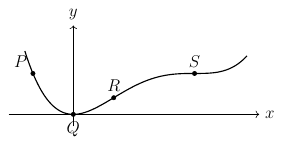
\includegraphics[width=0.6\linewidth]{data/calculus-figures/t4-labeled-curve.png}\end{center}
\begin{list}{}{\setlength{\leftmargin}{3em}\setlength{\labelwidth}{2.5em}\setlength{\itemsep}{0pt}\setlength{\topsep}{2pt}}
\item[(A)] $P$
\item[(B)] $Q$
\item[(C)] $R$
\item[(D)] $S$
\end{list}

\bigskip\noindent\textbf{TB40.}\ Use the labeled curve in the figure. At which labeled point is $\dfrac{dy}{dx}$ equal to zero and $\dfrac{d^2y}{dx^2}$ positive?
\begin{center}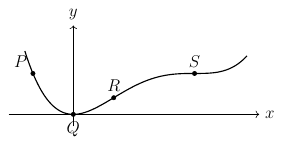
\includegraphics[width=0.6\linewidth]{data/calculus-figures/t4-labeled-curve.png}\end{center}
\begin{list}{}{\setlength{\leftmargin}{3em}\setlength{\labelwidth}{2.5em}\setlength{\itemsep}{0pt}\setlength{\topsep}{2pt}}
\item[(A)] $P$
\item[(B)] $Q$
\item[(C)] $R$
\item[(D)] $S$
\end{list}

\bigskip\noindent\textbf{TB41.}\ If $f(5) = 20$ and $f'(x) = \dfrac{x^2}{x+5}$, estimate $f(5.04)$ using the line tangent to $f$ at $x=5$.
\begin{list}{}{\setlength{\leftmargin}{3em}\setlength{\labelwidth}{2.5em}\setlength{\itemsep}{0pt}\setlength{\topsep}{2pt}}
\item[(A)] $19.9$
\item[(B)] $20.02$
\item[(C)] $20.08$
\item[(D)] $20.1$
\end{list}

\bigskip\noindent\textbf{TB42.}\ A local linear approximation for $f(x) = \sqrt{x^2+9}$ near $x=-4$ is
\begin{list}{}{\setlength{\leftmargin}{3em}\setlength{\labelwidth}{2.5em}\setlength{\itemsep}{0pt}\setlength{\topsep}{2pt}}
\item[(A)] $y = 5 - \dfrac{4}{5}(x-4)$
\item[(B)] $y = 5 + \dfrac{4}{5}(x-4)$
\item[(C)] $y = 5 - \dfrac{4}{5}(x+4)$
\item[(D)] $y = 4 - \dfrac{5}{4}(x+4)$
\end{list}

\end{document}
